% !TEX root =../dissertation.tex
\documentclass[./dissertation.tex]{subfiles}
\begin{document}

\chapter{Appendices}


\begin{table}[!ht]
  \centering
  \caption{Overview of Cell Tracking Challenge Datasets with Sample Images.}
  \label{tab:ctc_datasets_visual_summary}
  % \renewcommand{\arraystretch}{1.8} % Increase row spacing to accommodate images
  % \small % Optional: Adjust font size if needed

  % Adjust the 'lc' or use 'lp{width}' if specific alignment/wrapping is needed
  \begin{tabular}{|l|c|l|c|}
    \hline
    \textbf{2D Dataset Name} & \textbf{Sample Image}                                          & \textbf{3D Dataset Name} & \textbf{Sample Image}                                             \\ \hline

    % --- 2D Datasets ---
    BF-C2DL-HSC              & 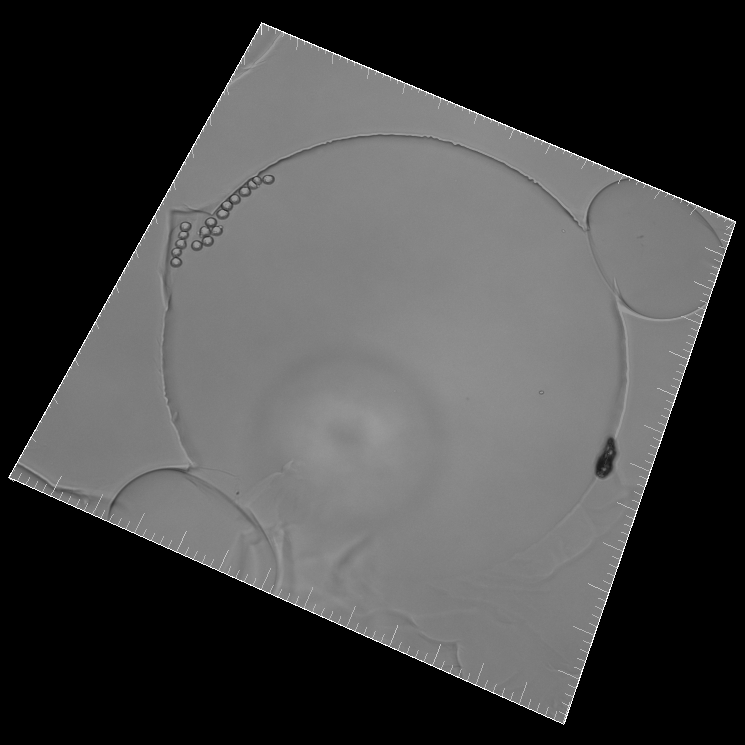
\includegraphics[width=2.3cm]{figures/ctc/BF-C2DL-HSC.png}     & Fluo-C3DH-A549           & 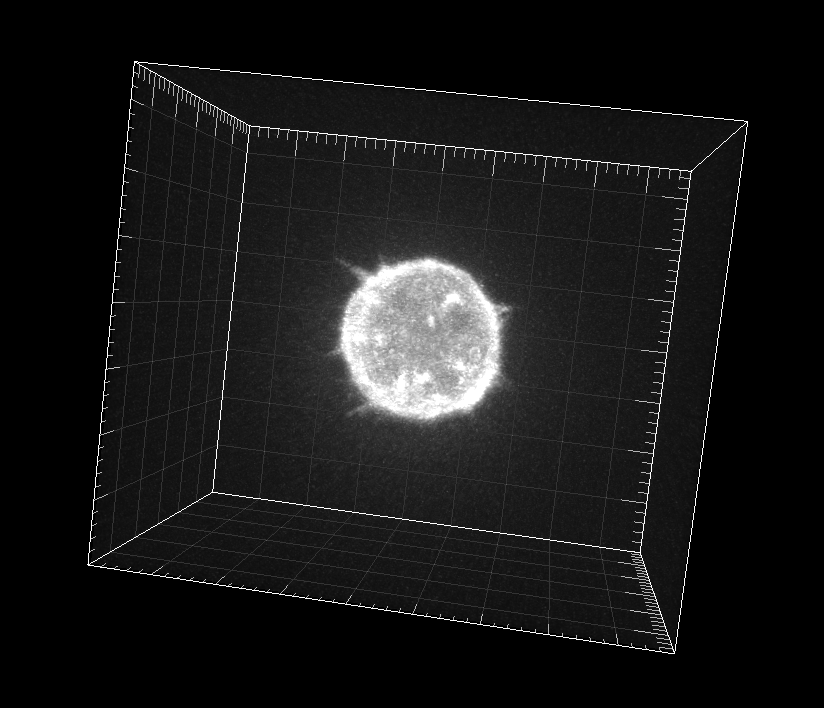
\includegraphics[width=2.3cm]{figures/ctc/Fluo-C3DH-A549.png}     \\ \hline
    BF-C2DL-MuSC             & 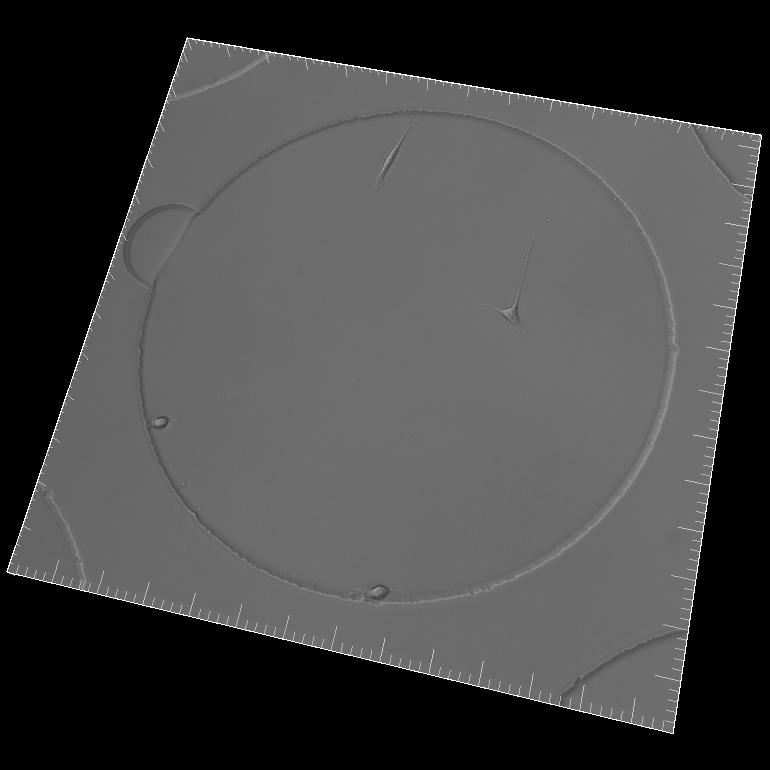
\includegraphics[width=2.3cm]{figures/ctc/BF-C2DL-MuSC.png}    & Fluo-C3DH-A549-SIM       & 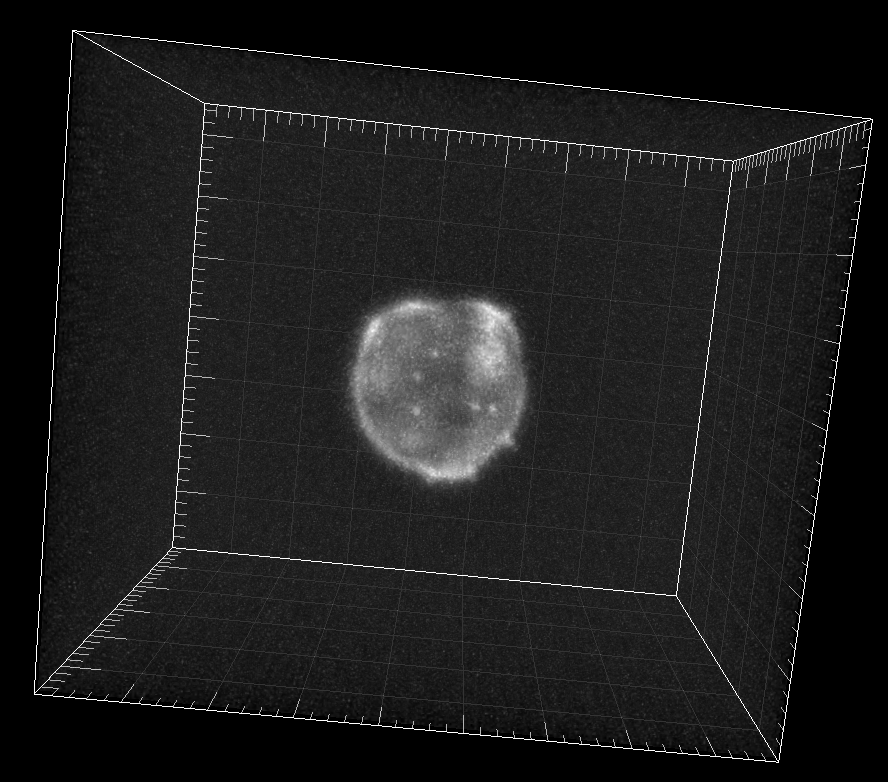
\includegraphics[width=2.3cm]{figures/ctc/Fluo-C3DH-A549-SIM.png} \\ \hline
    DIC-C2DH-HeLa            & 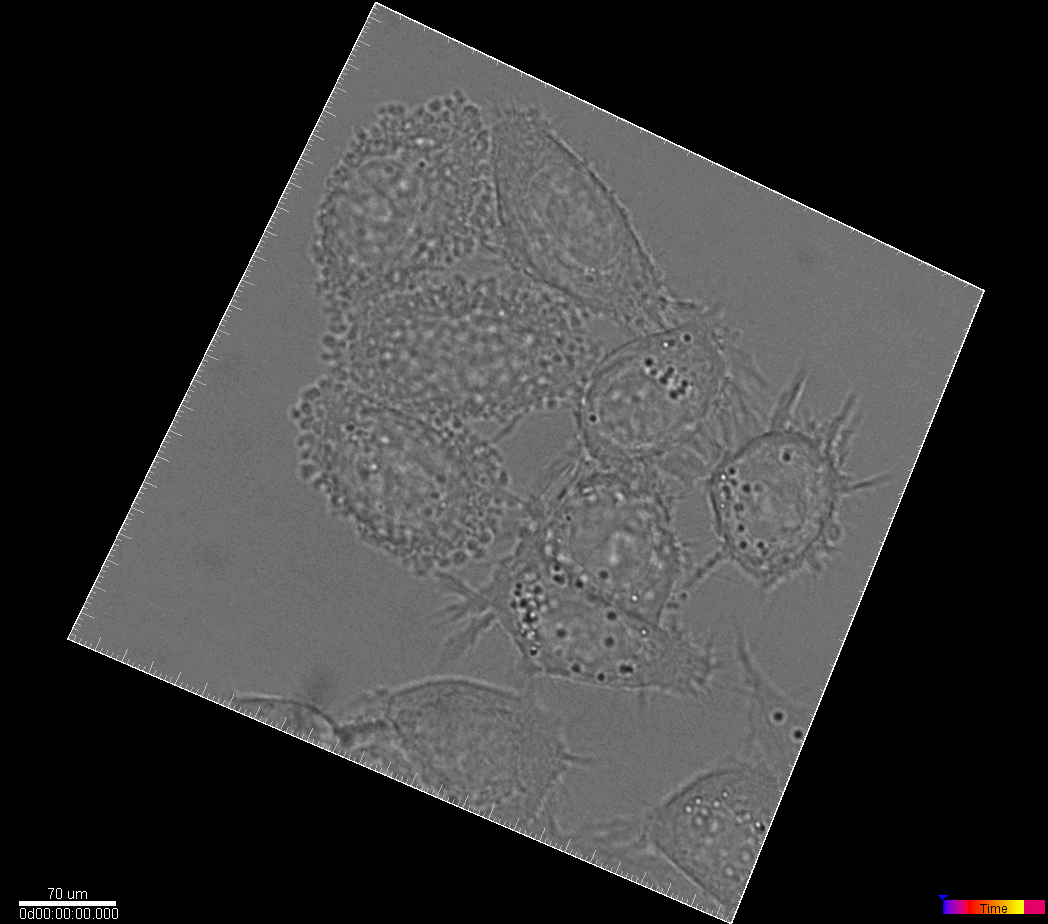
\includegraphics[width=2.3cm]{figures/ctc/DIC-C2DH-HeLa.png}   & Fluo-C3DH-H157           & 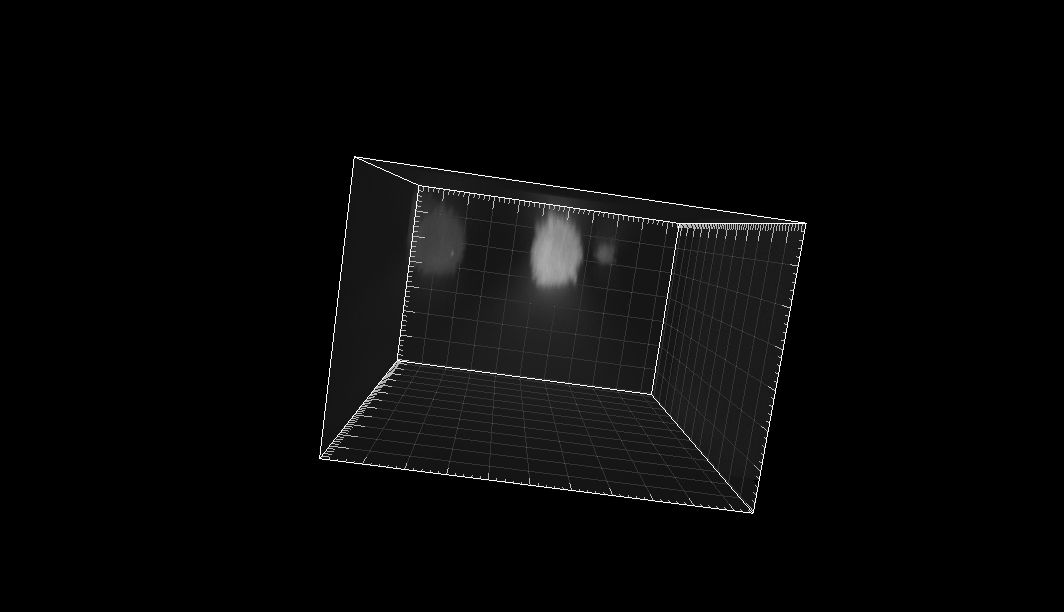
\includegraphics[width=2.3cm]{figures/ctc/Fluo-C3DH-H157.png}     \\ \hline
    Fluo-C2DL-Huh7           & 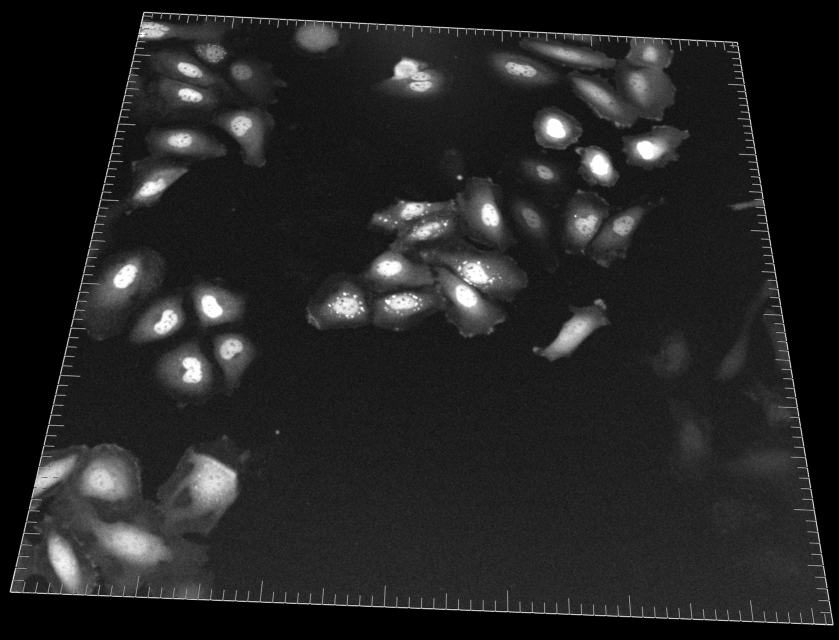
\includegraphics[width=2.3cm]{figures/ctc/Fluo-C2DL-Huh7.png}  & Fluo-C3DL-MDA231         & 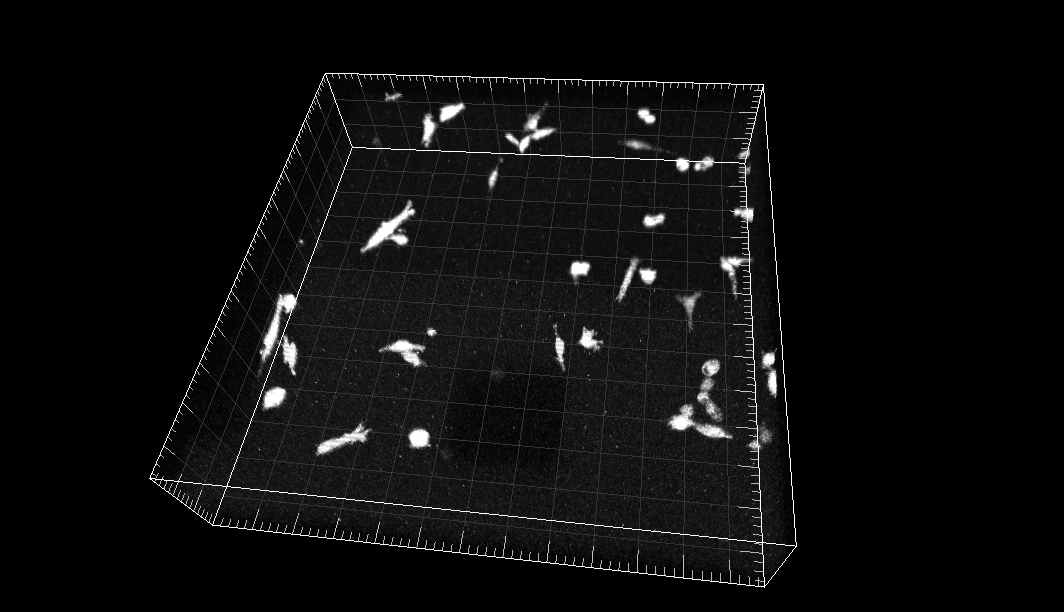
\includegraphics[width=2.3cm]{figures/ctc/Fluo-C3DL-MDA231.png}   \\ \hline
    Fluo-C2DL-MSC            & 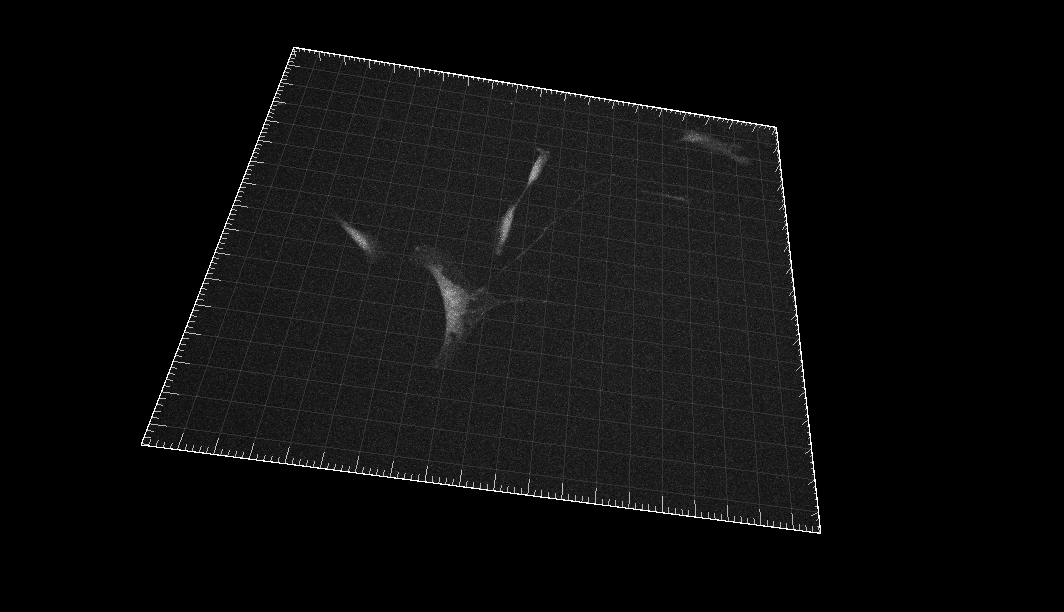
\includegraphics[width=2.3cm]{figures/ctc/Fluo-C2DL-MSC.png}   & Fluo-N3DH-CE             & 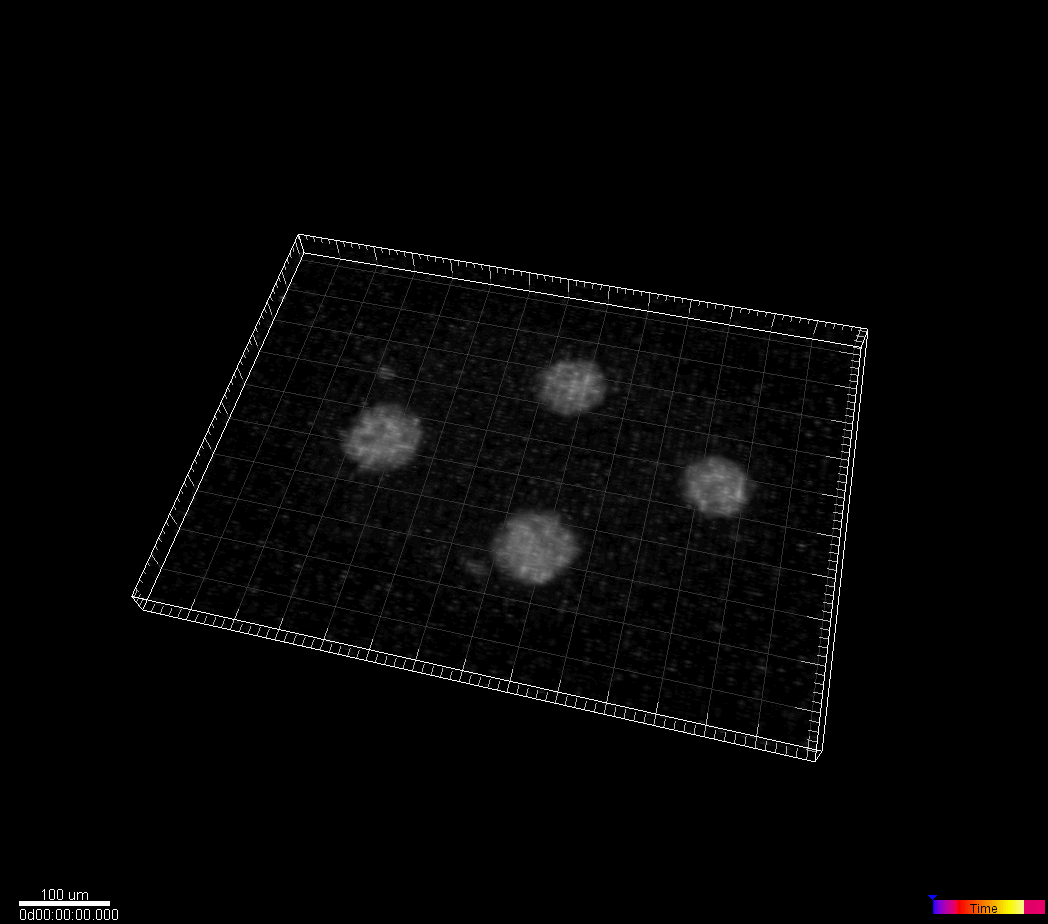
\includegraphics[width=2.3cm]{figures/ctc/Fluo-N3DH-CE.png}       \\ \hline
    Fluo-N2DH-GOWT1          & 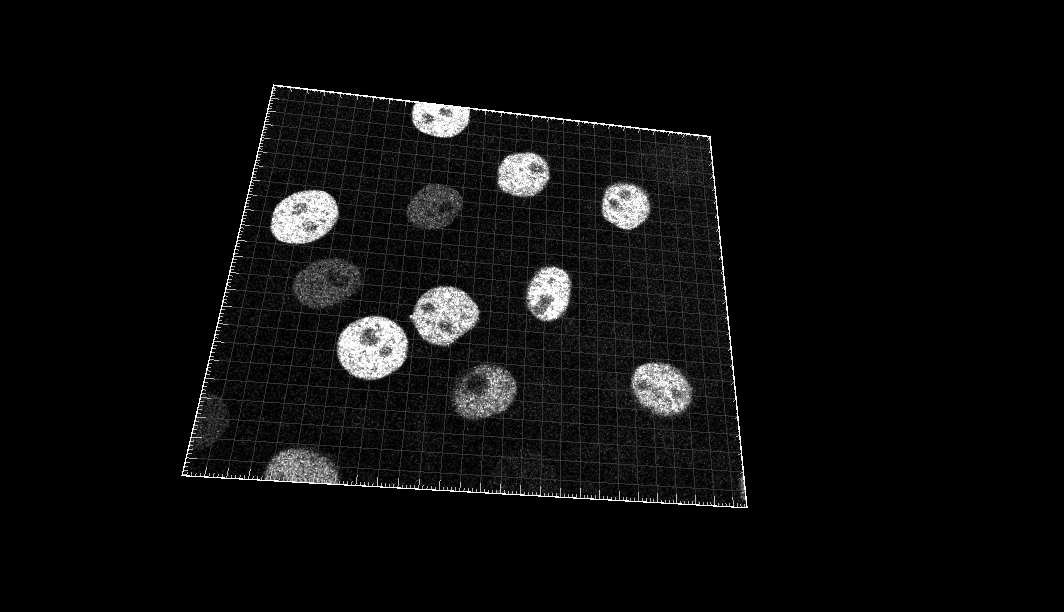
\includegraphics[width=2.3cm]{figures/ctc/Fluo-N2DH-GOWT1.png} & Fluo-N3DH-CHO            & 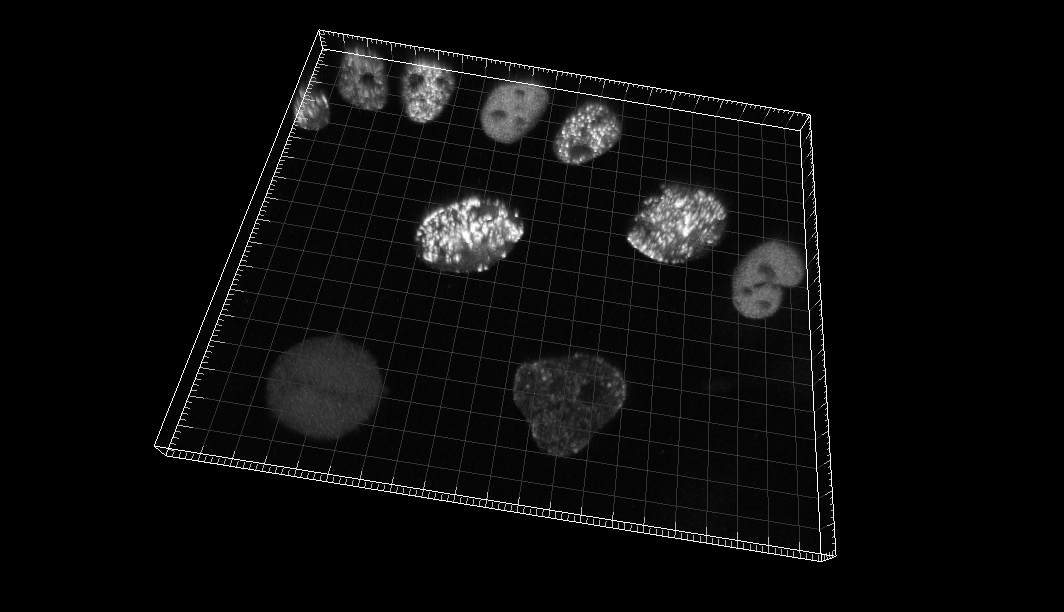
\includegraphics[width=2.3cm]{figures/ctc/Fluo-N3DH-CHO.png}      \\ \hline
    Fluo-N2DH-SIM            & 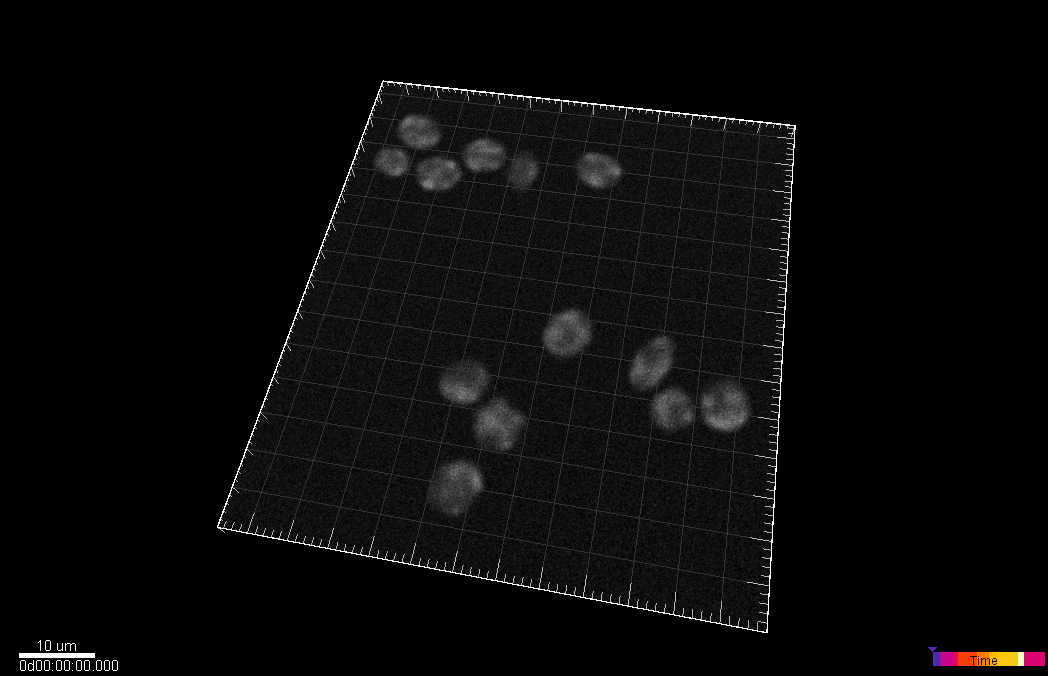
\includegraphics[width=2.3cm]{figures/ctc/Fluo-N2DH-SIM.png}   & Fluo-N3DH-SIM            & 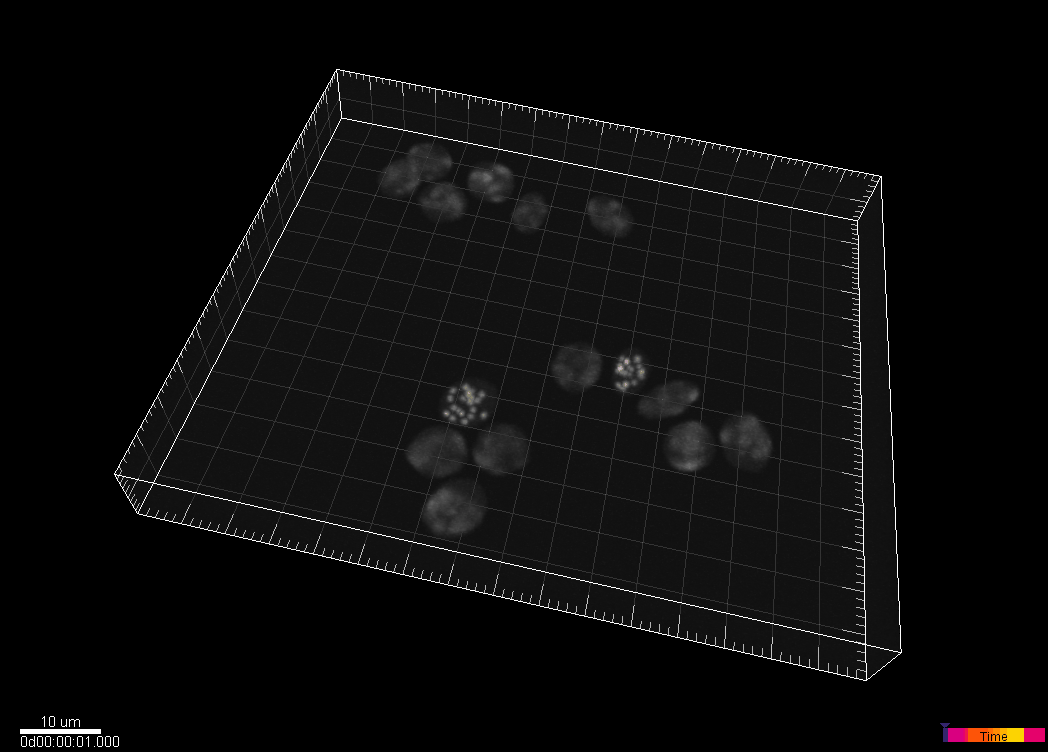
\includegraphics[width=2.3cm]{figures/ctc/Fluo-N3DH-SIM.png}      \\ \hline
    Fluo-N2DL-HeLa           & 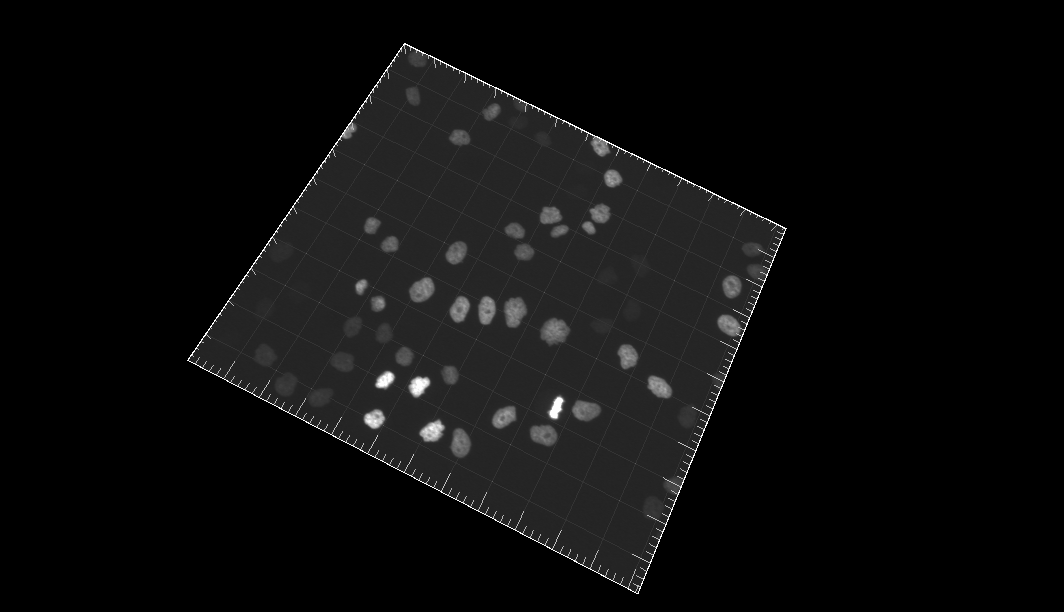
\includegraphics[width=2.3cm]{figures/ctc/Fluo-N2DL-HeLa.png}  & Fluo-N3DL-DRO            & 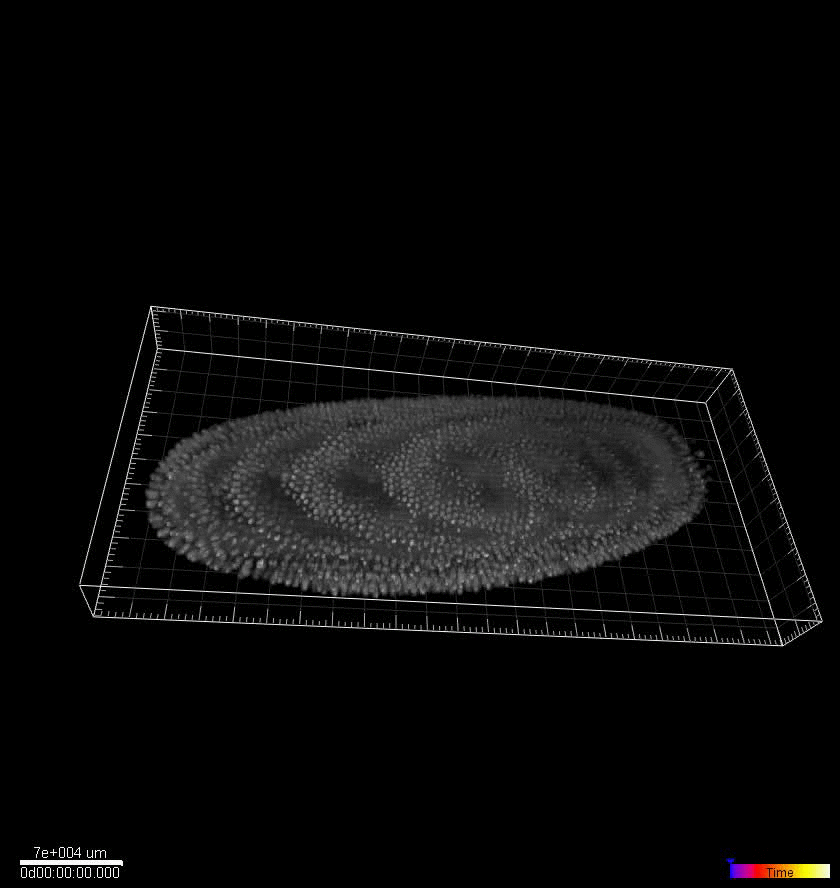
\includegraphics[width=2.3cm]{figures/ctc/Fluo-N3DL-DRO.png}      \\ \hline
    PhC-C2DH-U373            & 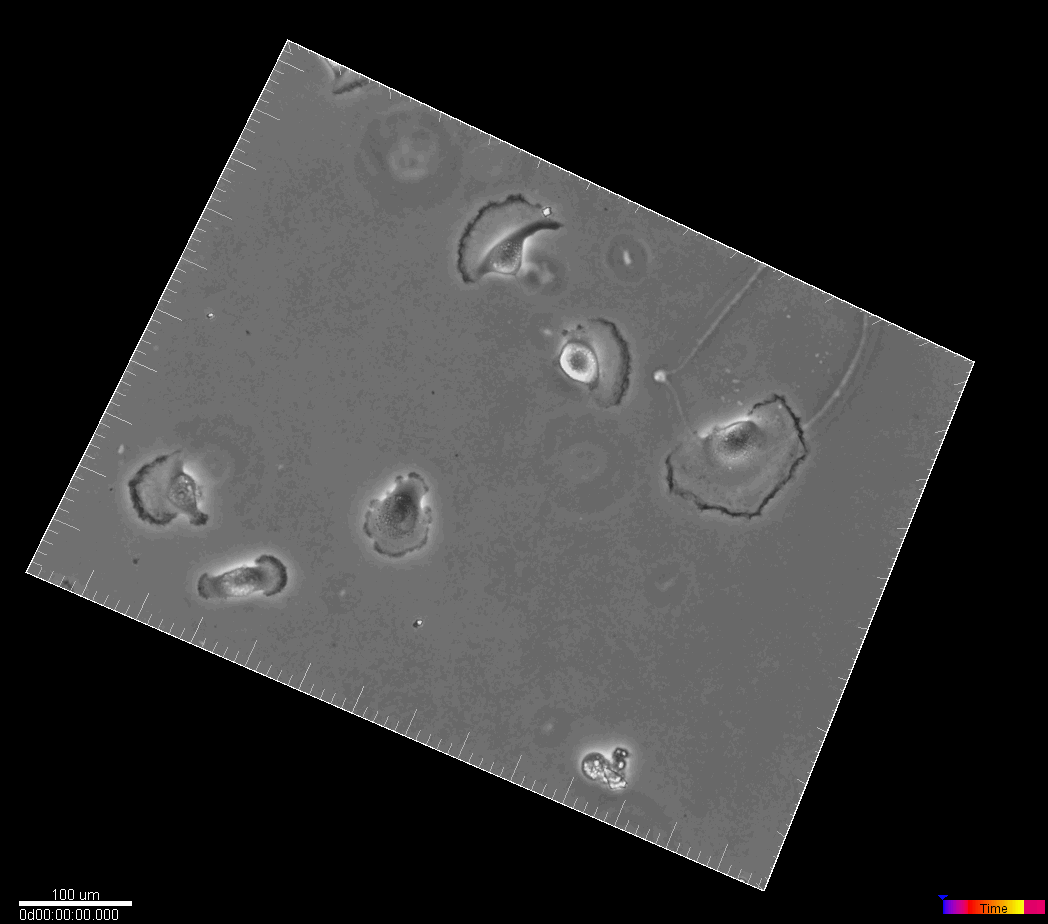
\includegraphics[width=2.3cm]{figures/ctc/PhC-C2DH-U373.png}   & Fluo-N3DL-TRIF           & 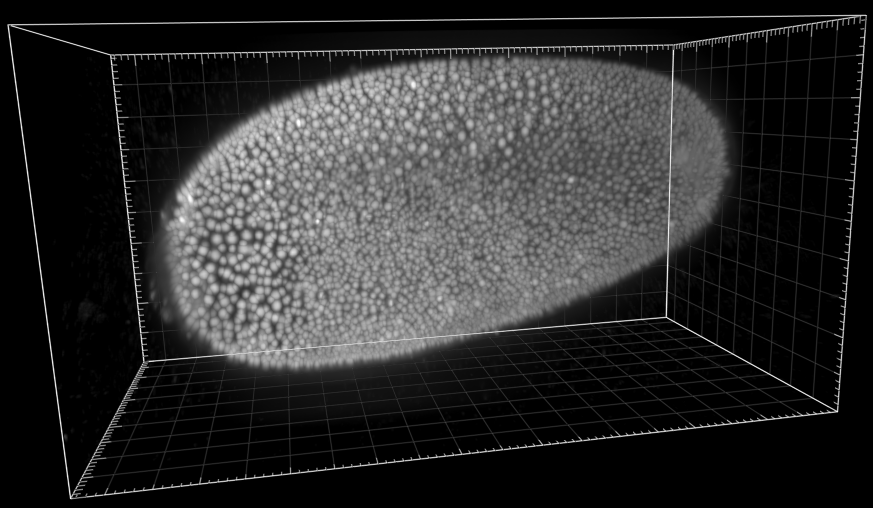
\includegraphics[width=2.3cm]{figures/ctc/Fluo-N3DL-TRIF.png}     \\ \hline
    PhC-C2DL-PSC             & 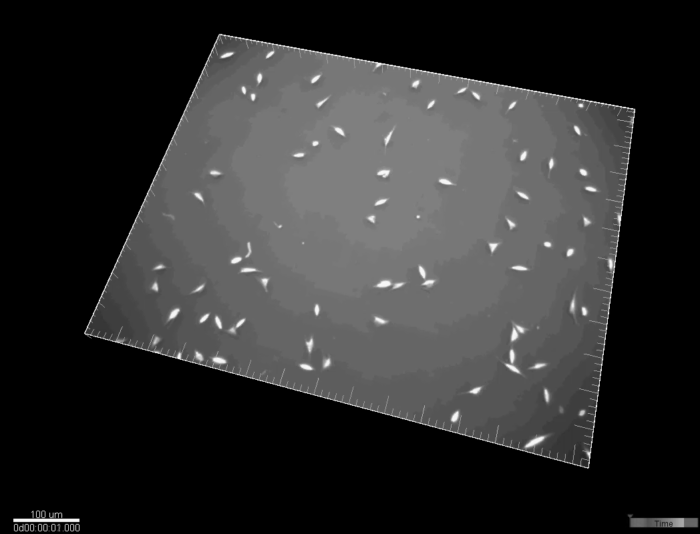
\includegraphics[width=2.3cm]{figures/ctc/PhC-C2DL-PSC.png}    & Fluo-N3DL-TRIC           & 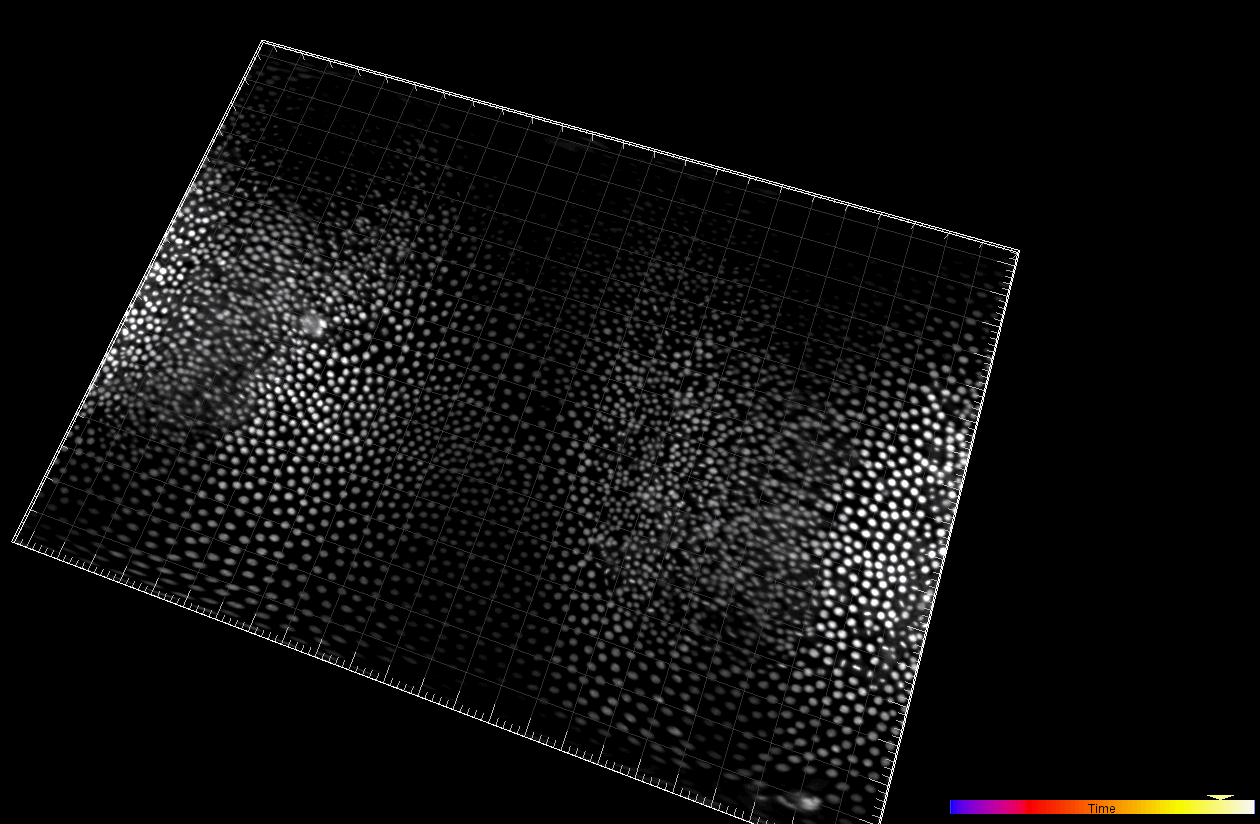
\includegraphics[width=2.3cm]{figures/ctc/Fluo-N3DL-TRIC.png}     \\ \hline
  \end{tabular}
  % \par % Add some space before notes
  % \vspace{1ex}
  % \footnotesize % Notes in smaller font
  % Note: Image paths assume files are located in a 'figures/datasets/' subdirectory relative to your main LaTeX file. Adjust the path and `width` parameter as needed for your document layout. `\addlinespace` requires the `booktabs` package.
\end{table}
\begin{table}[!ht]
  \centering
  \caption{CellPose Performance on 2D Datasets}
  \label{tbl:cellpose_2d_segmentation}
  \renewcommand{\arraystretch}{1.2}
  \small
  \begin{tabular}{|l|c|c|c|c|c|c|c|c|c|c|}
    \hline
    % \toprule
    \textbf{dataset name}     & \rotatebox{90}{\textbf{BF-C2DL-HSC}} & \rotatebox{90}{\textbf{BF-C2DL-MuSC}} & \rotatebox{90}{\textbf{DIC-C2DH-HeLa}} & \rotatebox{90}{\textbf{Fluo-C2DL-Huh7}} & \rotatebox{90}{\textbf{Fluo-C2DL-MSC}} & \rotatebox{90}{\textbf{Fluo-N2DH-GOWT1}} & \rotatebox{90}{\textbf{Fluo-N2DH-SIM+}} & \rotatebox{90}{\textbf{Fluo-N2DL-HeLa}} & \rotatebox{90}{\textbf{PhC-C2DH-U373}} & \rotatebox{90}{\textbf{PhC-C2DL-PSC}} \\ \hline
    % \midrule \hline
    cyto3                     & 0.98                                 & 0.95                                  & 0.36                                   & 0.60                                    & 0.90                                   & 0.89                                     & 0.82                                    & 0.75                                    & 0.87                                   & 0.87                                  \\ \hline
    nuclei                    & 0.99                                 & 0.99                                  & 0.36                                   & 0.60                                    & 0.89                                   & 0.86                                     & 0.80                                    & 0.75                                    & 0.87                                   & 0.90                                  \\ \hline
    cyto2\_cp3                & 0.94                                 & 0.95                                  & 0.35                                   & 0.60                                    & 0.89                                   & 0.87                                     & 0.82                                    & 0.74                                    & 0.85                                   & 0.87                                  \\ \hline
    tissuenet\_cp3            & 0.98                                 & 0.97                                  & 0.36                                   & 0.59                                    & 0.89                                   & 0.86                                     & 0.80                                    & 0.75                                    & 0.87                                   & 0.91                                  \\ \hline
    livecell\_cp3             & 0.98                                 & 0.99                                  & 0.36                                   & 0.59                                    & 0.89                                   & 0.86                                     & 0.80                                    & 0.75                                    & 0.87                                   & 0.91                                  \\ \hline
    yeast\_PhC\_cp3           & 0.98                                 & 0.98                                  & 0.34                                   & 0.59                                    & 0.84                                   & 0.86                                     & 0.71                                    & 0.75                                    & 0.86                                   & 0.88                                  \\ \hline
    yeast\_BF\_cp3            & 0.99                                 & 0.99                                  & 0.36                                   & 0.60                                    & 0.89                                   & 0.86                                     & 0.79                                    & 0.73                                    & 0.87                                   & 0.91                                  \\ \hline
    bact\_phase\_cp3          & 0.97                                 & 0.97                                  & 0.35                                   & 0.59                                    & 0.89                                   & 0.86                                     & 0.79                                    & 0.73                                    & 0.86                                   & 0.89                                  \\ \hline
    bact\_fluor\_cp3          & 0.93                                 & 0.95                                  & 0.33                                   & 0.59                                    & 0.89                                   & 0.86                                     & 0.79                                    & 0.73                                    & 0.84                                   & 0.89                                  \\ \hline
    deepbacs\_cp3             & 0.99                                 & 0.99                                  & 0.36                                   & 0.60                                    & 0.89                                   & 0.86                                     & 0.80                                    & 0.75                                    & 0.87                                   & 0.90                                  \\ \hline
    cyto2                     & 0.95                                 & 0.96                                  & 0.36                                   & 0.60                                    & 0.90                                   & 0.88                                     & 0.82                                    & 0.73                                    & 0.86                                   & 0.86                                  \\ \hline
    cyto                      & 0.97                                 & 0.97                                  & 0.35                                   & 0.59                                    & 0.89                                   & 0.87                                     & 0.80                                    & 0.72                                    & 0.84                                   & 0.86                                  \\ \hline
    CPx                       & 0.97                                 & 0.98                                  & 0.34                                   & 0.59                                    & 0.89                                   & 0.88                                     & 0.80                                    & 0.73                                    & 0.86                                   & 0.90                                  \\ \hline
    neurips\_grayscale\_cyto2 & 0.99                                 & 0.98                                  & 0.35                                   & 0.60                                    & 0.89                                   & 0.88                                     & 0.89                                    & 0.67                                    & 0.87                                   & 0.91                                  \\ \hline
    CP                        & 0.97                                 & 0.95                                  & 0.35                                   & 0.60                                    & 0.89                                   & 0.88                                     & 0.81                                    & 0.72                                    & 0.86                                   & 0.89                                  \\ \hline
    TN1                       & 0.98                                 & 0.99                                  & 0.36                                   & 0.60                                    & 0.89                                   & 0.86                                     & 0.80                                    & 0.75                                    & 0.86                                   & 0.91                                  \\ \hline
    TN2                       & 0.99                                 & 0.98                                  & 0.36                                   & 0.59                                    & 0.89                                   & 0.86                                     & 0.80                                    & 0.75                                    & 0.87                                   & 0.91                                  \\ \hline
    TN3                       & 0.99                                 & 0.99                                  & 0.36                                   & 0.60                                    & 0.89                                   & 0.86                                     & 0.80                                    & 0.75                                    & 0.87                                   & 0.91                                  \\ \hline
    LC1                       & 0.99                                 & 0.99                                  & 0.27                                   & 0.59                                    & 0.89                                   & 0.89                                     & 0.79                                    & 0.75                                    & 0.87                                   & 0.91                                  \\ \hline
    LC2                       & 0.96                                 & 0.97                                  & 0.36                                   & 0.60                                    & 0.89                                   & 0.86                                     & 0.79                                    & 0.75                                    & 0.85                                   & 0.90                                  \\ \hline
    LC3                       & 0.98                                 & 0.97                                  & 0.33                                   & 0.60                                    & 0.89                                   & 0.86                                     & 0.80                                    & 0.74                                    & 0.82                                   & 0.85                                  \\ \hline
    LC4                       & 0.95                                 & 0.98                                  & 0.36                                   & 0.59                                    & 0.89                                   & 0.86                                     & 0.80                                    & 0.75                                    & 0.87                                   & 0.83                                  \\ \hline
    % \bottomrule
  \end{tabular}
\end{table}

% Second Table (PlantSeg Performance)
\begin{table}[!ht]
  \centering
  \caption{PlantSeg Performance on 2D Datasets}
  \label{tbl:plantseg_2d_segmentation}
  \renewcommand{\arraystretch}{1.2}
  \small
  \begin{tabular}{|l|c|c|c|c|c|c|c|c|c|c|}
    \hline
    % \toprule
    \textbf{dataset name}                    & \rotatebox{90}{\textbf{BF-C2DL-HSC}} & \rotatebox{90}{\textbf{BF-C2DL-MuSC}} & \rotatebox{90}{\textbf{DIC-C2DH-HeLa}} & \rotatebox{90}{\textbf{Fluo-C2DL-Huh7}} & \rotatebox{90}{\textbf{Fluo-C2DL-MSC}} & \rotatebox{90}{\textbf{Fluo-N2DH-GOWT1}} & \rotatebox{90}{\textbf{Fluo-N2DH-SIM+}} & \rotatebox{90}{\textbf{Fluo-N2DL-HeLa}} & \rotatebox{90}{\textbf{PhC-C2DH-U373}} & \rotatebox{90}{\textbf{PhC-C2DL-PSC}} \\ \hline
    % \midrule
    confocal\_2D\_unet\_ovules\_ds2x         & 0.99                                 & 0.99                                  & 0.36                                   & 0.59                                    & 0.89                                   & 0.86                                     & 0.80                                    & 0.75                                    & 0.87                                   & 0.91                                  \\ \hline
    lightsheet\_2D\_unet\_root\_ds1x         & 0.99                                 & 0.99                                  & 0.36                                   & 0.59                                    & 0.89                                   & 0.86                                     & 0.80                                    & 0.75                                    & 0.87                                   & 0.91                                  \\ \hline
    lightsheet\_2D\_unet\_root\_nuclei\_ds1x & 0.99                                 & 0.99                                  & 0.36                                   & 0.59                                    & 0.89                                   & 0.86                                     & 0.80                                    & 0.75                                    & 0.87                                   & 0.91                                  \\ \hline
    confocal\_2D\_unet\_sa\_meristem\_cells  & 0.99                                 & 0.99                                  & 0.36                                   & 0.59                                    & 0.89                                   & 0.86                                     & 0.80                                    & 0.75                                    & 0.87                                   & 0.91                                  \\ \hline
    % \bottomrule
  \end{tabular}
\end{table}

% First Table (CellPose Performance on 3D datasets)
\begin{table}[!ht]
  \centering
  \caption{CellPose Performance on 3D Datasets}
  \label{tbl:cellpose_3d_segmentation}
  \small
  \begin{tabular}{|l|c|c|c|c|c|c|}
    % \toprule
    \hline
    \textbf{dataset\_name}    & \rotatebox{90}{\textbf{Fluo-C3DH-A549}} & \rotatebox{90}{\textbf{Fluo-C3DH-A549-SIM}} & \rotatebox{90}{\textbf{Fluo-C3DH-H157}} & \rotatebox{90}{\textbf{Fluo-N3DH-CE}} & \rotatebox{90}{\textbf{Fluo-N3DH-CHO}} & \rotatebox{90}{\textbf{Fluo-N3DH-SIM+}} \\ \hline
    % \midrule \hline
    cyto3                     & 0.96                                    & 0.97                                        & 0.93                                    & 0.80                                  & 0.83                                   & 0.92                                    \\ \hline
    nuclei                    & 0.96                                    & 0.97                                        & 0.93                                    & 0.80                                  & 0.84                                   & 0.93                                    \\ \hline
    cyto2\_cp3                & 0.97                                    & 0.97                                        & 0.93                                    & 0.80                                  & 0.79                                   & 0.93                                    \\ \hline
    tissuenet\_cp3            & 0.96                                    & 0.97                                        & 0.93                                    & 0.80                                  & 0.84                                   & 0.93                                    \\ \hline
    livecell\_cp3             & 0.96                                    & 0.95                                        & 0.93                                    & 0.80                                  & 0.84                                   & 0.93                                    \\ \hline
    yeast\_PhC\_cp3           & 0.92                                    & 0.93                                        & 0.88                                    & 0.68                                  & 0.84                                   & 0.86                                    \\ \hline
    yeast\_BF\_cp3            & 0.95                                    & 0.97                                        & 0.92                                    & 0.80                                  & 0.83                                   & 0.88                                    \\ \hline
    bact\_phase\_cp3          & 0.96                                    & 0.97                                        & 0.93                                    & 0.79                                  & 0.83                                   & 0.93                                    \\ \hline
    bact\_fluor\_cp3          & 0.96                                    & 0.97                                        & 0.93                                    & 0.80                                  & 0.83                                   & 0.93                                    \\ \hline
    deepbacs\_cp3             & 0.96                                    & 0.97                                        & 0.93                                    & 0.80                                  & 0.84                                   & 0.93                                    \\ \hline
    cyto2                     & 0.96                                    & 0.98                                        & 0.93                                    & 0.80                                  & 0.84                                   & 0.94                                    \\ \hline
    cyto                      & 0.96                                    & 0.97                                        & 0.93                                    & 0.80                                  & 0.82                                   & 0.93                                    \\ \hline
    CPx                       & 0.98                                    & 0.99                                        & 0.93                                    & 0.80                                  & 0.83                                   & 0.93                                    \\ \hline
    neurips\_grayscale\_cyto2 & 0.97                                    & 0.98                                        & 0.93                                    & 0.73                                  & 0.82                                   & 0.92                                    \\ \hline
    CP                        & 0.98                                    & 0.99                                        & 0.93                                    & 0.79                                  & 0.82                                   & 0.93                                    \\ \hline
    TN1                       & 0.96                                    & 0.97                                        & 0.93                                    & 0.80                                  & 0.84                                   & 0.93                                    \\ \hline
    TN2                       & 0.96                                    & 0.97                                        & 0.93                                    & 0.80                                  & 0.84                                   & 0.93                                    \\ \hline
    TN3                       & 0.96                                    & 0.99                                        & 0.93                                    & 0.80                                  & 0.84                                   & 0.93                                    \\ \hline
    LC1                       & 0.86                                    & 0.97                                        & 0.92                                    & 0.80                                  & 0.82                                   & 0.92                                    \\ \hline
    LC2                       & 0.96                                    & 0.97                                        & 0.93                                    & 0.80                                  & 0.84                                   & 0.93                                    \\ \hline
    LC3                       & 0.96                                    & 0.13                                        & 0.93                                    & 0.79                                  & 0.82                                   & 0.30                                    \\ \hline
    LC4                       & 0.96                                    & 0.97                                        & 0.93                                    & 0.80                                  & 0.84                                   & 0.93                                    \\ \hline
    % \bottomrule
  \end{tabular}
\end{table}

% Second Table (PlantSeg Performance on 3D datasets)
\begin{table}[!ht]
  \centering
  \caption{PlantSeg Performance on 3D Datasets}
  \label{tbl:plantseg_3d_segmentation}
  \small
  \begin{tabular}{|l|c|c|c|c|c|c|}
    \hline
    % \toprule
    \textbf{dataset\_name}                    & \rotatebox{90}{\textbf{Fluo-C3DH-A549}} & \rotatebox{90}{\textbf{Fluo-C3DH-A549-SIM}} & \rotatebox{90}{\textbf{Fluo-C3DH-H157}} & \rotatebox{90}{\textbf{Fluo-N3DH-CE}} & \rotatebox{90}{\textbf{Fluo-N3DH-CHO}} & \rotatebox{90}{\textbf{Fluo-N3DH-SIM+}} \\ \hline
    % \midrule \hline
    generic\_confocal\_3D\_unet               & 0.96                                    & 0.97                                        & 0.88                                    & 0.78                                  & 0.84                                   & ---                                     \\ \hline
    generic\_light\_sheet\_3D\_unet           & 0.96                                    & 0.97                                        & 0.88                                    & 0.78                                  & 0.84                                   & ---                                     \\ \hline
    confocal\_3D\_unet\_ovules\_ds1x          & 0.96                                    & 0.97                                        & 0.88                                    & 0.78                                  & 0.84                                   & ---                                     \\ \hline
    confocal\_3D\_unet\_ovules\_ds2x          & 0.96                                    & 0.97                                        & 0.88                                    & 0.78                                  & 0.84                                   & ---                                     \\ \hline
    confocal\_3D\_unet\_ovules\_ds3x          & 0.96                                    & 0.97                                        & 0.88                                    & ---                                   & 0.84                                   & ---                                     \\ \hline
    lightsheet\_3D\_unet\_root\_ds1x          & 0.96                                    & 0.97                                        & 0.88                                    & ---                                   & 0.84                                   & ---                                     \\ \hline
    lightsheet\_3D\_unet\_root\_ds2x          & 0.96                                    & 0.97                                        & 0.88                                    & ---                                   & 0.84                                   & ---                                     \\ \hline
    lightsheet\_3D\_unet\_root\_ds3x          & 0.96                                    & 0.97                                        & 0.88                                    & ---                                   & 0.84                                   & ---                                     \\ \hline
    lightsheet\_3D\_unet\_root\_nuclei\_ds1x  & 0.96                                    & 0.97                                        & 0.88                                    & ---                                   & 0.84                                   & ---                                     \\ \hline
    confocal\_3D\_unet\_sa\_meristem\_cells   & 0.96                                    & 0.97                                        & 0.88                                    & ---                                   & 0.84                                   & ---                                     \\ \hline
    confocal\_3D\_unet\_mouse\_embryo\_nuclei & 0.96                                    & 0.97                                        & 0.88                                    & ---                                   & 0.84                                   & ---                                     \\ \hline
    PlantSeg\_3Dnuc\_platinum                 & 0.96                                    & 0.97                                        & 0.88                                    & ---                                   & 0.84                                   & ---                                     \\ \hline
    % \bottomrule
  \end{tabular}
\end{table}
% \lipsum[7]

\begin{figure}
  \centering
  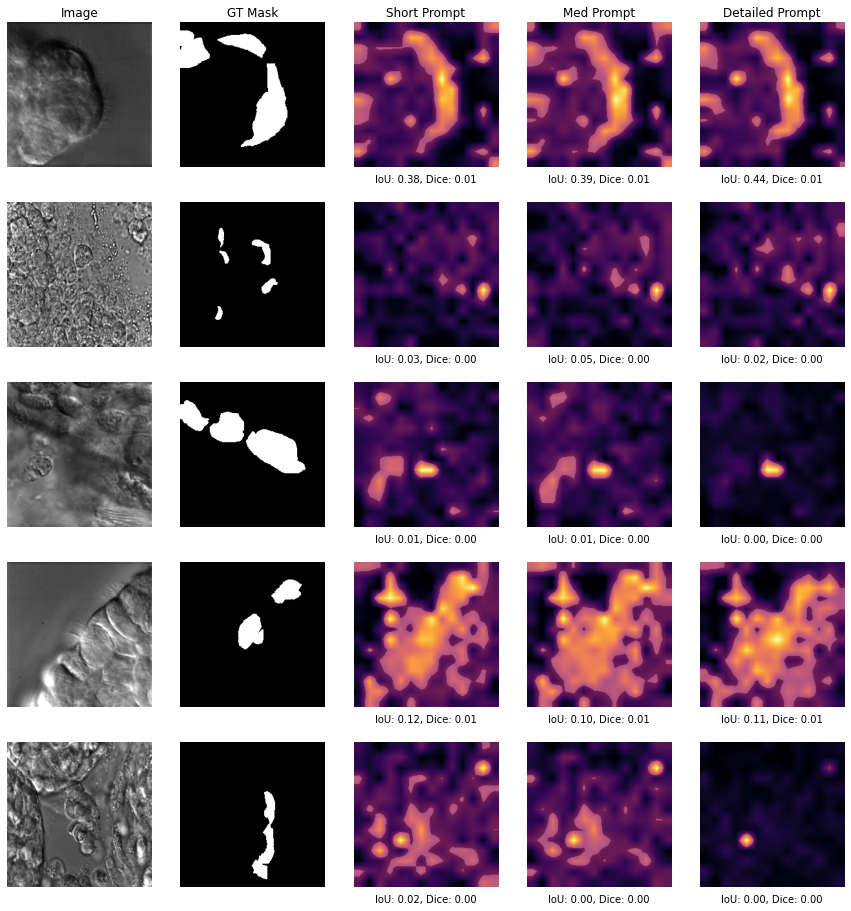
\includegraphics[width=\textwidth]{figures/sam/fine-tuned 1ep with mask short caption th 0.4.png}
  \caption{Improved ciliary region localization after fine-tuning BiomedCLIP for one epoch using masked images with short captions.}
  \label{fig:fine_tuned_mask_short_ep1}
\end{figure}

\begin{figure}
  \centering
  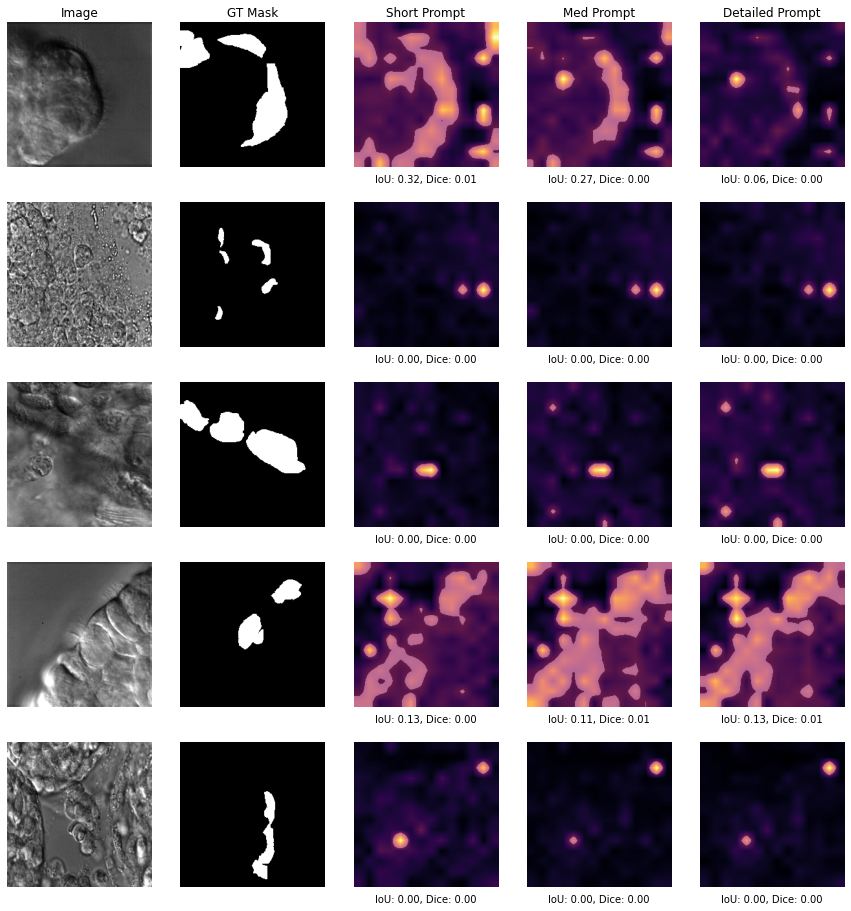
\includegraphics[width=\textwidth]{figures/sam/fine-tuned masks small train short desc ep5.png}
  \caption{Effective and balanced localization achieved by fine-tuning BiomedCLIP with a reduced dataset size (small train) using masked images and short captions for 5 epochs.}
  \label{fig:fine_tuned_mask_small_short_ep5}
\end{figure}

\begin{figure}
  \centering
  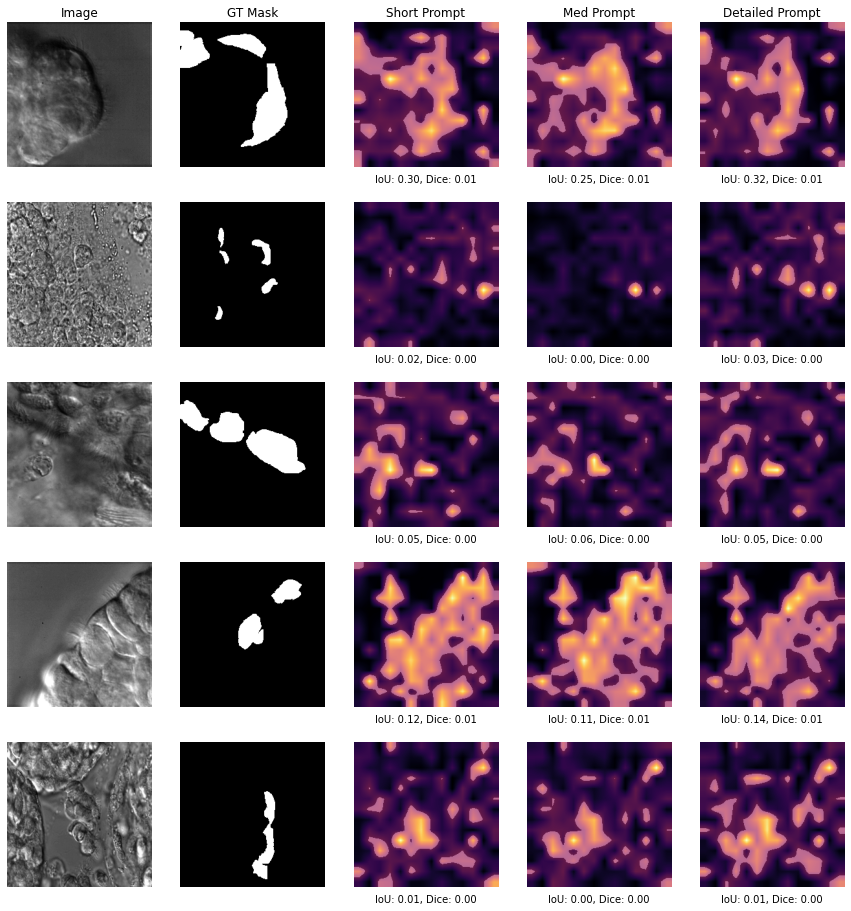
\includegraphics[width=\textwidth]{figures/sam/train with long captions.png}
  \caption{Localization results demonstrating increased flexibility but higher false positives when fine-tuning BiomedCLIP using long captions.}
  \label{fig:train_long_captions}
\end{figure}

\begin{figure}
  \centering
  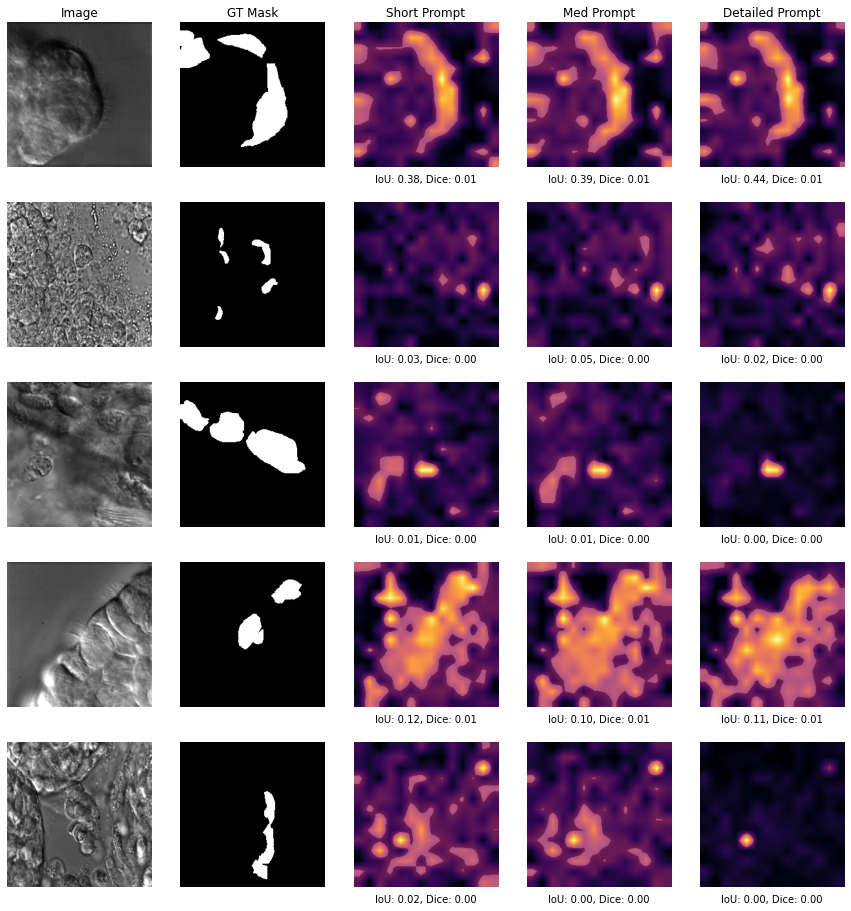
\includegraphics[width=\textwidth]{figures/sam/fine-tuned with mask th 0.4.png}
  \caption{Localization impact of higher temperature (\(\tau = 0.4\)) during fine-tuning, resulting in blurred similarity distributions and compromised accuracy.}
  \label{fig:fine_tuned_with_mask_th_0_4}
\end{figure}

\end{document}
